\documentclass{article} 		% see Section 1.3
% See lines 11-22 of alounsburymacros.sty for a different/better way of including packages. 
% I leave these here merely to point out the sections where I use these
% packages. 
\usepackage{amsfonts, amsmath, amssymb, amsthm}	% math symbols, environments, etc. 
\usepackage{graphicx, float} 	% for inserting pictures
	\graphicspath{{images/}} 		% set the path from which LaTeX pulls images
\usepackage{mathrsfs} 			% see Theorem 1, Section 3.1
\usepackage{kbordermatrix} 		% see Section 3.2.4
	\renewcommand{\kbldelim}{(} % left delimiter, default is [
	\renewcommand{\kbrdelim}{)} % right delimiter, default is ]
\usepackage{units, xcolor} 		% see Section 5
\usepackage{fancyvrb} 			% see Section 5.4
\usepackage{verse}				% see Section 5.5
\usepackage{alounsburymacros}		% includes macros from alounsburymacros.sty
% ignore this stuff------------
\usepackage{footnote}
	\makesavenoteenv{tabular}
\usepackage{hyperref}
\hypersetup{
	colorlinks=true,
	linkcolor=blue,
	urlcolor=blue,
}
%------------------------------

\newcommand{\sddots}{\rotatebox{-30}{$\ddots$}} % see Section 3.2.4

\begin{document}
\begin{titlepage}
	\title{\bfseries \LaTeX\ for Undergraduates\footnote{
			Throughout this paper, there are some commands from the accompanying \texttt{alounsburymacros} package, but I'm going to forgo further reference to \texttt{alounsburymacros.sty}. If you use a command from this tutorial in another document and it says the command is undefined, you probably need to install \texttt{alounsburymacros} and include it in the preamble. 
		}
	}
	\author{Andrew Lounsbury}
	\date{February 27, 2024}
	\maketitle
	
	\vspace{1.5in}

	To put a title on a simple homework assignment, you only need lines \texttt{31}-\texttt{37} in the code (\texttt{LaTeX\_for\_Undergraduates.tex}) instead of an entire \texttt{titlepage}, but you don't necessarily have to use this method. You can put the title, your name, and the date on the paper however you'd like. \\

	As you read this, use the keyboard shortcut Ctrl + F to search for specific things in the code so that you can compare the code precisely to what's being printed. 
	\vspace{1.5in}
	\begin{center}
		
\includegraphics[width=0.15\textwidth]{TechSignatureSeal_Purple_RGB.jpg}
	\end{center}
\end{titlepage}

\tableofcontents

\newpage
\section{Setting Up} \label{sec:setting-up}
\subsection{MiKTeX} \label{subsec:miktex}
Click \href{https://miktex.org/download}{here} to download MiKTeX. Install it to the default directory. When it asks if MiKTeX should install packages on the fly, say \textbf{yes}.

\subsection{\LaTeX\ Editors: Visual Studio Code} \label{subsec:editors}
I recommend Visual Studio Code for Windows users and (maybe) Mac users.\footnote{
	If you can't or don't want to use VS Code, see \href{https://en.wikipedia.org/wiki/Comparison_of_TeX_editors}{here} and \href{https://tex.stackexchange.com/questions/339/latex-editors-ides}{here}.
} 
To download the User Installer for VS Code, click \href{https://code.visualstudio.com/download}{here}. When it gives the option to add the ``Open with Code'' action to file and directory context menus, \textbf{check both} boxes. \par
Open \texttt{LaTeX\_for\_Undergraduates.tex} in VS Code. With the 
\includegraphics[scale=0.06]{marketplace.png} button on the left sidebar, install the following:
\begin{enumerate}
	\item[]
	LaTeX Workshop

	\item[]
	Code Spell Checker

	\item[]
	Notepad++ keymap
\end{enumerate}

Initially, there is a wide scrollbar that shows a zoomed-out image of your code. You can toggle this under \texttt{View -> Show Minimap}. \par
Click the gear in the bottom left, select \texttt{Settings}
, and change the following:\footnote{
	There is a button at the top right that opens a \texttt{json} file with all overridden settings. 
}
\begin{center}
	\begin{tabular}{|l|l|}
		\hline
		Editor: Word Wrap & \textbf{on} \\ \hline
		Auto Find in Selection & \textbf{multiline} \\ \hline
		LaTeX Workshop $>$ Message $>$ Error: Show & \textbf{uncheck} the box \\ \hline
		Workbench: Startup Editor & \textbf{none} \\ \hline
	\end{tabular}
\end{center}

Try building the file with the green button in the top-right. \par
Windows users may receive an error in the bottom left regarding a file \texttt{perl.exe} from a programming language called \textbf{Perl}. 
Click \href{https://www.perl.org/get.html}{here} to download Perl. There is a choice between \textit{Strawberry Perl} and \textit{ActiveState Perl}. A Stack Exchange page said that ActiveState Perl is better for beginners, so it's probably fine to download that one. \par
Now, you may need to add the path to your Perl installation to the Path variable. If so, search your computer for the option to edit your \textit{Environment Variables} in your \textit{System Properties}. Select \texttt{Environment Variables...} Under \textit{System variables}, select \textbf{Path} and click \texttt{Edit...}. 
\begin{center}
	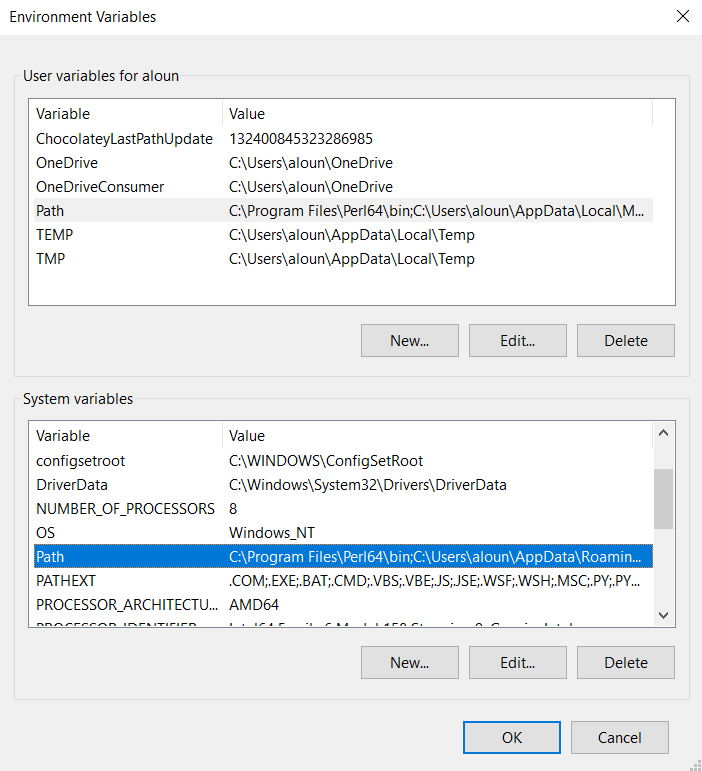
\includegraphics[width=0.765\textwidth]{perl1.png}
\end{center}
Add the path to your Perl installation with the \texttt{New} button on the right:
\begin{center}
	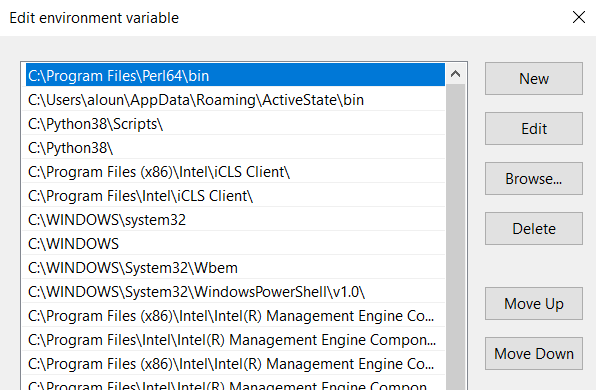
\includegraphics[width=0.765\textwidth]{perl2crop.png}
\end{center}
Try building the file again to ensure everything works properly.\footnote{
	Producing the result of \LaTeX\ code is generally referred to as ``building the file,'' but I will occasionally refer to this as ``compiling the file.'' I mean the former by the latter. 
} 
It will likely take longer than usual because it has to install the necessary packages and generate the auxiliary files for the first time and because this is an eighteen-page document. Be sure to press the button in the top right with the magnifying glass to open the \texttt{pdf} and see the result of the compilation. 

\subsection{Creating a Document in VS Code} \label{subsec:creating-document}
Create new files and open files under \texttt{File}. Regarding the three buttons 
\includegraphics[scale=0.08]{compiling.png} in the top-right corner, the play button on the left builds the file, the middle button with the magnifying glass displays the \texttt{pdf}, and the button on the right splits the editor so that you can open multiple files or open a duplicate view of the same file.\footnote{
	I've noticed that when I close my laptop with a \texttt{pdf} open, that \texttt{pdf} will no longer update when I rebuild. Closing and reopening the \texttt{pdf} seems to consistently fix this. 
} 
Note, however, that LaTeX Workshop has a setting that builds your code every time you save. \par
View error messages by clicking the icons in the bottom-left corner. 
\begin{center}
	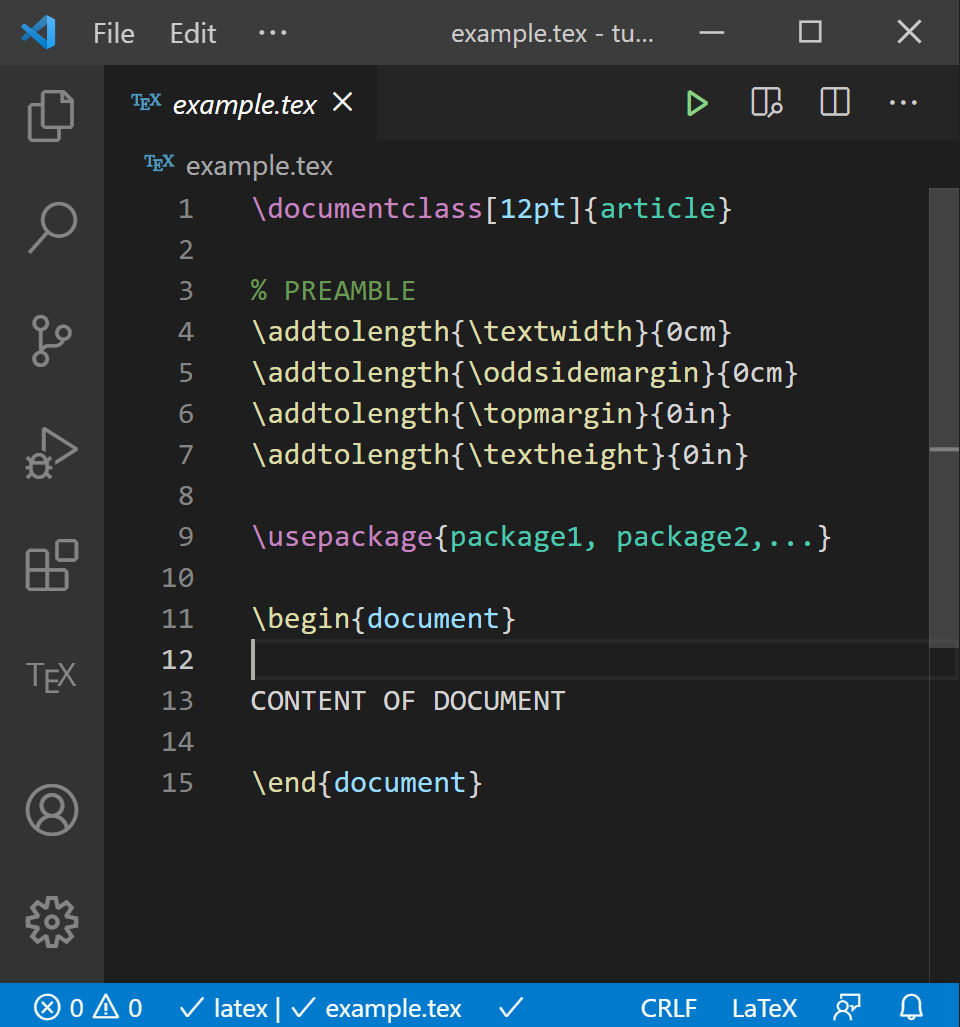
\includegraphics[width=0.6\textwidth]{creatingDocument.png}
\end{center}

The font size \texttt{[12pt]} is optional and may be set to sizes other than \texttt{12}. The \href{https://ctan.org/pkg/article}{\texttt{article}} class is for regular documents.\footnote{
	The \href{https://ctan.org/pkg/beamer}{\texttt{beamer}} class allows us to make presentation slides and posters in \LaTeX. 
}
The preamble is everything between \verb$\documentclass{article}$ and \verb$\begin{document}$, in other words, your margins and text dimensions,\footnote{
	An alternative method of setting these values is \texttt{\textbackslash setlength\{\textbackslash lengthname\}\{}\opt{dimension}\texttt{\}}. 
} 
which are optional, and your packages. \p
Regarding the content of the document, writing in \LaTeX\ can generally be summarized as (1) typing regular text, (2) typing math with \texttt{\$\dots\$}, (3) displaying math with \verb$\[...\]$, and (4) learning commands and environments as you need them. Any text contained in \verb$\begin{$\opt{env-name}\verb$}...\end{$\opt{env-name}\verb$}$ is in the \opt{env-name} environment. 

\subsection{Keyboard Shortcuts in VS Code} \label{subsec:shortcuts}
Remember to make ample use of the following shortcuts. 

\begin{center}
	\begin{tabular}{|c||l||l|}
		\hline
		\textbf{Source}\footnote{
			VSC = VS Code; LW = \LaTeX\ Workshop; N++ = Notepad++ keymap \p
			\cby{\textbf{NOTE}}: These \LaTeX\ Workshop shortcuts must be added in the shortcut menu. 
		} & \textbf{Shortcut} & \textbf{Action} \\ \hline\hline
		VSC & Ctrl + A & highlight all \\ \hline
		N++ & Ctrl + D & duplicate \\ \hline
		LW & Ctrl + E & select current environment \\ \hline
		VSC & Ctrl + F \& Ctrl + H & search \& replace \\ \hline
		LW & Ctrl + K & kill compiler process \\ \hline
		N++ & Ctrl + Q & toggle comments \\ \hline
		LW & Ctrl + T & toggle between \texttt{\textbackslash[\dots\textbackslash]} and \\
		& & the \texttt{equation*} environment \\ \hline
		LW & Ctrl + W & wrap in environment \\ \hline
		VSC & Ctrl + Z \& Ctrl + Y & undo \& redo (even autocompletion) \\ \hline
		VSC & Double Click & highlight string \\ \hline
		VSC & Highlight + Delimiter & wrap in \texttt{\{}\dots\texttt{\}}, \texttt{(}\dots\texttt{)}, \texttt{[}\dots\texttt{]}, \texttt{\$}\dots\texttt{\$} \\ \hline
		VSC & Shift + Click & highlight everything between the \\ 
		& 			  & text cursor and your mouse cursor \\ \hline
		VSC & Tab \& Shift + Tab & tab/untab multiple lines; \\
		& 				   & next/previous argument in a macro \\ \hline
		VSC & Tab or Enter & autocomplete suggested text \\ \hline
		VSC & Shift + Enter & prevent an autocompletion \\ \hline
	\end{tabular}
\end{center}

These save lots of time. If your editor doesn't have them, you may want to look through your settings and add these shortcuts or change them if they're different from what you want them to be. In VS Code, you can view your keyboard shortcuts in the settings at the bottom-left.\footnote{
	There is a button at the top right in the shortcuts menu that opens the \texttt{json} file with all overridden shortcuts. 
}

\subsubsection{Autocompletion} \label{subsubsec:autocompletion}
VS Code allows us to autocomplete any string of regular text provided the string has already been typed into the document once. It doesn't give the option to autocomplete ``Nullstellensatz'' in this document because we haven't typed it yet, but if we type ``Nullstellensatz'' again, it gives us the option. \par
For commands, autocompletion doesn't trigger in new, unsaved files nor for commands that haven't already been typed \textit{and saved} into the document once. Upon typing \verb$\msum$ for the first time, we don't have the option to autocomplete it and successively enter its arguments, but upon adding the three \verb${...}$ to the first instance, saving the document, and typing \verb$\msum$ a second time, we can press Tab and VS Code automatically types \verb$\msum{$\rule[-0.5ex]{1pt}{2.5ex}\verb$}{}{}$ with the braces ready and the text cursor inside the first set of braces. 

\section{Text} \label{sec:text}
Regular text is said to be in paragraph mode. 
\subsection{Formatting Text} \label{subsec:formatting-text}
Comment things out with \texttt{\%}.\footnote{
	There is a \texttt{comment} environment in the \texttt{verbatim} package for creating block comments. The benefit of this is that we can minimize environments in VS Code so that we don't have to constantly scroll through code we're not reading. We could otherwise highlight the multiple lines we want to comment out and press Ctrl + Q (or an equivalent shortcut). 
} \par
% This sentence is not in the pdf. 
Create a new line without indentation using \verb$\\$. \\
Create a new paragraph with indentation either with \verb$\par$ or by leaving an empty line in the code.\footnote{
	See lines \texttt{26}-\texttt{31} of \texttt{alounsburymacros.sty} for a way to fix indentation of \texttt{\textbackslash par} and empty lines in \texttt{enumerate} and \texttt{itemize} environments. 
} \par
An empty line with a 
%
comment symbol will not create a new line. See code. 

\noindent
We can stop the indentation on an empty line like this.\footnote{
	We wouldn't use \texttt{\textbackslash par} unless we specifically wanted the indentation.
}

It's good to use these in such a way that makes your code look similar to what's being printed. Using \verb$\\$ along with an empty line will create an empty line in both your code and your document. \\

\noindent
This will produce \underline{underlined} text. \\
This will produce \textit{italicized} text. \\
This will produce \textbf{boldface} text. \\
This will produce \textsc{small caps} text. \\
This will produce \texttt{typewriter (teletype)} font. \\
This will reproduce \verb%whatever's between the $'s% in \texttt{teletype} font.\footnote{
	Various characters will work in place of the \texttt{\%}. For instance, the \texttt{\%}'s on line \texttt{186} can be replaced with \texttt{\$}'s or even the characters \texttt{0} through \texttt{9}, \texttt{[}, or \texttt{)}. 
} \\

Changing the $\langle\textit{font-size}\rangle$ option in \verb%\documentclass[%$\langle\textit{font-size}\rangle$\verb%]{article}% will affect the way the following sizes work. For instance, \verb$[12pt]$ makes \verb$\huge$ and \verb$\Huge$ appear the same. \\

\noindent
English is not a {\tiny finite state language}. \\
English is not a {\footnotesize finite state language}. \\
English is not a {\small finite state language}. \\
English is not a finite state language. \\
English is not a {\large finite state language}. \\
English is not a {\Large finite state language}. \\
English is not a {\LARGE finite state language}. \\
English is not a {\huge finite state language}. \\
English is not a {\Huge finite state language}. 

\begin{center}
	This is centered.
\end{center}
%
\begin{flushleft}
	This is left-justified.
\end{flushleft}
%
\begin{flushright}
	This is right-justified.
\end{flushright}
%
You can insert horizontal space \hspace{1in} like this, or 
insert vertical space 
\vspace{0.25in} \\
like this. 

\subsection{Lists} \label{subsec:lists}
\begin{enumerate}
	\item[1.]
	This is \texttt{enumerate}.\footnote{
		The \href{https://ctan.org/pkg/enumitem}{\texttt{enumitem}} package provides additional functionality for \texttt{enumerate}.
	}
	
	\item[label \#2]
	Though it numbers items automatically, it's good to label the items so that you can tell the difference between all the \verb$\item$'s in your code. Note that you can change the labels with brackets. 
	
	\item[3.]
	\begin{enumerate}
		\item% a
		Once-nested \texttt{enumerate} environment 
		
		\item% b
			\begin{enumerate}
				\item% i
				Twice-nested
				
				\item% ii
				\begin{enumerate}
					\item% A
					Thrice-nested
					
					\item% B
					This is the maximum number of times you can nest them. 
				\end{enumerate}
			\end{enumerate}

	\end{enumerate}
\end{enumerate}

\begin{itemize}
	\item
	This is \texttt{itemize}. 
	\item% dot
	Good labeling for \texttt{itemize} might be ``dot'', ``dash'', ``star'', ``point,'' but the utility of this depends on whether you put \verb$\item$ on its own line or the same line as your text. 
	
	\item% dot
	\begin{itemize}
		\item% dash
		Once-nested \texttt{itemize} environment 
		
		\item% dash
			\begin{itemize}
				\item% star
				Twice-nested
				
				\item% star
				\begin{itemize}
					\item % point
					Thrice-nested
					
					\item% point
					This is the maximum number of times you can nest them. 
					
				\end{itemize}
			\end{itemize}
	\end{itemize}
\end{itemize}

\begin{tabular}{|l||c||r|}
	\hline
	There is also & the \texttt{tabular} & environment. \\ \hline\hline
	It's like an & array without & math mode. \\ \hline
	Each column alignment & must be & indicated. \\ \hline
	\texttt{l} = left-justified & & \\ \hline
	& \texttt{c} = centered & \\ \hline
	& & \texttt{r} = right-justified \\ \hline
\end{tabular}

\newpage
\section{Math} \label{sec:math}
Mathematical text is said to be in math mode. 
\subsection{Formatting Math} \label{subsec:formatting-math}
$Math mode is italicized by default$. \\
This will produce $\text{regular text with whitespace.}$ \\
This will produce $\textbf{bold text with whitespace.}$ \\
This will produce $\textit{italicized text with whitespace.}$ \\
This will produce $\textsc{small caps text with whitespace.}$ \\
This will produce $\mathbf{boldface math without whitespace}$.\footnote{
	See Notation \ref{notation:bold} for a possible alternative.
} \\
This will produce $\mathrm{roman (nonitalicized\ serif\ font) text without whitespace}$. 

\begin{theorem*}[Commands \& Trouble-Shooting]
	Regarding \LaTeX\ commands, there is plenty of information at your disposal on the internet. You will likely be able to solve most of the problems you encounter and find commands and packages you need by searching for them on the internet. 
\end{theorem*}
\begin{proof}
	Search for a list of commands such as \href{https://oeis.org/wiki/List_of_LaTeX_mathematical_symbols}{this} or \href{http://tug.ctan.org/info/symbols/comprehensive/symbols-a4.pdf}{this}. Search for a package that suites your needs. Search for the error your compiler is giving. Stack Exchange, Overleaf, and Wikibooks are fantastic resources. \par
	Under the \LaTeX\ menu on the left sidebar in VS Code, there are two Snippet panels with a myriad of symbols to browse through. Relying on these menus is ill-advised, but being aware of them may still be worthwhile. Here are just a few commands worth noting: 
	\begin{enumerate}
		\item[1.]
		$\sin\theta_1 = \cos\theta_2 = \max\{0,1\} = \min\{1,2\} = 3 \bmod 2 = \sqrt[4]{1} = \pm 1$

		\item[2.]
		$\exists \ell \in \cap_{i=1}^n A_i$ such that $f \circ g(\ell) = \gcd(7,\ell) = \mathrm{lcm}(7,\ell) = 10 = \underbrace{1 + \cdots + 1}_{10 \tms}$

		\item[3.]
		\begin{enumerate}
			\item% a 
			$\dim V = \mathrm{rank}(T) + \dim\Null(T)$, where $T \in \mathcal{L}(V,W)$

			\item% b
			$|\mathcal{P}(S)| = 2^{|S|}$
		\end{enumerate}

		\item[4.]
		$\mathscr{L}\{f(t - a)\mathscr{U}(t - a)\}=e^{-as}F(s)$ % mathrsfs package

		\item[5.]
		$\mseti{x_n}{n}{1} \subset \R$ is such that $\inf x_n \le \sup x_n$ and $\liminf x_n \le \limsup x_n$. \qedhere % forcing the \qedsymbol to appear in the display
	\end{enumerate}
\end{proof}

\begin{notation}
	\texttt{\{\dots\}} are required around subscripts and superscripts with more than one character (except for commands such as $\infty$, greek letters, etc.)  
\end{notation}

\begin{claim*}
	The statement $x_m^{n+1} +     x_{m+1}^n     \approx 2^\pi \not< 8 \le 2^\infty$ is 
	\begin{enumerate}
		\item
			in inline math mode and 
		\item
			has none of the extra white-space from the code. 
	\end{enumerate}
\end{claim*}
\begin{proof}[Proof of (1)]
	Lorem ipsum dolor sit amet, consectetur adipiscing elit, sed do eiusmod tempor incididunt ut labore et dolore magna aliqua. 
	\renewcommand{\qedsymbol}{}
\end{proof}
\begin{proof}[Proof of (2)]
	Note that we temporarily changed the \verb$\qedsymbol$ in the previous \texttt{proof} environment so that it wouldn't show up twice. Also, note that we can change the title of any environment with brackets. 
\end{proof}

\begin{proposition*}[Display-Math Mode]
	The summation
	\[
		\sum_{i=1}^n i^2 = \f{n(n+1)(2n+1)}{6} \in \Theta(n^3)
	\]
	is in display-math mode. Note that the first letters of commands for capital Greek letters are capitalized and that there are some lowercase Greek letters with variations whose commands begin with \textnormal{\texttt{var}}, such as $\varphi$ and $\varepsilon$. 
\end{proposition*}
\begin{proof}
	Omitted
\end{proof}

\begin{corollary*}[\texttt{equation} \& \texttt{multline}]
	Let $I \subseteq \ring$ be an ideal, where $k$ is an algebraically closed field. Then, 
	\begin{equation} \label{eq:null}
		\IV{I} = \sqrt{I},
	\end{equation}
	and 
	\begin{multline} \label{eq:fx}
		f_x = 3x^2y^4 + 6xy^5 + 3y^6 - 8x^3y^2 - 18x^2y^3 - 12xy^4 - 2y^5 \\
		+ 5x^4 + 12x^3y + 9x^2y^2 + 2xy^3
	\end{multline}
	Equations (\ref{eq:null}) and (\ref{eq:fx}) are respectively in the \textnormal{\texttt{equation}} and \textnormal{\texttt{multline}} environments, which number single lines of display-math. The \textnormal{\texttt{multline}} environment is useful for splitting single lines. 
\end{corollary*}
\begin{proof}
	Omitted
\end{proof}

\begin{notation}[Extensible Block Delimiters] \label{notation:extensible}
	The commands \verb$\left$ and \verb$\right$ resize the succeeding character to fit whatever's between them. The null delimiters \verb$\left.$ and \verb$\right.$ respectively leave the left and right character blank, but there must be both a \verb$\left$\opt{something} and a \verb$\right$\opt{something}. Note that we can create extensible angle brackets with \verb$\left<$ and \verb$\right>$: 
	\[
		\left<\f{x}{2},\f{y}{2}\right> = 
		\set*{h_1\left(\f{x}{2}\right) + h_2\left(\f{y}{2}\right) \Mid h_1,h_2 \in \ring}. 
	\]
\end{notation}

\begin{notation}[Punctuation]
	When display-math mode ends a phrase, the punctuation \textit{must} be inside the display. For instance, it is true that 
	\[
		(0,1) = \bigcup_{n=2}^\infty \mpar{0 + \f{1}{n}, 1 - \f{1}{n}} \neq \varnothing, 
	\]
	but it may be true that $\gamma \in \Q$ or that $\gamma \notin \Q$. Hence, we may write $\gamma \stackrel{?}\in \Q$. 
\end{notation}

\begin{notation}[Readability]
	Separate long strings of equalities over several lines of code. It's better to write 
	\begin{verbatim}
		15
		= 10 + 5
		= 3 + 7 + 5
		= 1 + 2 + 3 + 4 + 5
	\end{verbatim}
rather than 
\begin{verbatim}
	15 = 10 + 5 = 3 + 7 + 5 = 1 + 2 + 3 + 4 + 5
\end{verbatim}
Also, \verb${$ and \verb$}$ don't have to appear on the same line. For example, 
\begin{Verbatim}
\mbrack{
	\mpar{
		\f{e^x + e^{-x}}{2}
	}
	\mpar{
		\f{e^x - e^{-x}}{2}
	}
}
\end{Verbatim}
makes it much easier to see where everything is. 
\end{notation}

\begin{notation}[Such That]
	There are two ways to say ``such that''	in a set definition. If $I,J \subseteq \ring$ are ideals, where $k$ is an algebraically closed field, then 
	\[
		\sqrt{I} = \{f \in \ring : f^m \in I \fs m \in \N\}, 
	\]
	and 
	\[
		I:J = \{f \in \ring \mid fg \in I \fa g \in J\}.\footnote{
			This is not the $\vert$ character on your keyboard. It's \texttt{\textbackslash mid}. Also, note the use of \texttt{\textbackslash set} and the extensible \texttt{\textbackslash Mid} in Notation \ref{notation:extensible}. 
		}
	\]
\end{notation}

\begin{notation}[Forcing Display-Math]
	Various notations get scrunched up in inline math: 
	$\sum_{i=1}^n$, 
	$\prod_{i=1}^n$, 
	$\bigcap_{i=1}^n$, 
	$\bigcup_{i=1}^n$, 
	$\lim_{n \to \infty}$, 
	$\sup_n (b_n)$, 
	$\int_a^b$, 
	$\max_n\{\delta_n\}$, etc. \par
	We can often override this by putting \verb$\limits$
	after each command.
	So, we can write 
	$\sum\limits_{i=1}^n$, 
	$\prod\limits_{i=1}^n$, 
	$\bigcap\limits_{i=1}^n$, 
	$\bigcup\limits_{i=1}^n$, 
	$\lim\limits_{n \to \infty}$,  
	$\sup\limits_n(b_n)$, 
	$\max\limits_n\{\delta_n\}$. \par
	Integrals can be put in \verb$\displaystyle$: $\dint{a}{b}$, but \verb$\limits$ does provide an alternative way of writing them: $\int\limits_a^b$. \par
	This is not necessary when these are being displayed, except for \verb$\int\limits$. 
	\[
		\sum_{i=1}^n,~ 
		\prod_{i=1}^n,~ 
		\bigcap_{i=1}^n,~ 
		\bigcup_{i=1}^n,~
		\lim_{n \to \infty},~
		\sup_n(b_n),~
		\max_n\{\delta_n\},~
		\int_a^b, \et
		 \int\limits_a^b
	\]
\end{notation}

\begin{notation}[Bold Math Symbols] \label{notation:bold}
	In math mode, mathematical symbols will not be affected by \verb$\mathbf{}$, as in $\mathbf{\sin\pi \notin \{1, 2, 3\}}$. To remedy this, use \verb$\boldsymbol{}$ as in $\boldsymbol{\sin\pi \notin \{1, 2, 3\}}$. \par
	When nesting block delimiters inside of each other, it is often beneficial to use an abbreviation of \verb$\boldsymbol$ to bold the outer delimiters. For instance, $g^{-1}\bs((c,d)\bs)$ is a little better than $g^{-1}((c,d))$. 
\end{notation}

\subsection{Displaying Multiple Lines of Math and Trees} \label{subsec:multiple-lines}
There are several ways to display multiple lines of math. Some environments have predefined numbering. Add a \texttt{*} when you \texttt{begin} and \texttt{end} the environment to remove numbering. Note that \verb$\\$ creates a new row. 

\subsubsection{\texttt{gather}} \label{subsubsec:gather}
The \texttt{gather} environment is like a multiline \texttt{center} environment that is in math mode by default. Let $V_1,\dots,V_n \subseteq k^n$ be varieties, where $k$ is an algebraically closed field. Then, 
\begin{gather}
	\varnothing \subseteq V_1 \subseteq \cdots \subseteq V_n \\
	\Rightarrow \mathbf{I}(\varnothing) \supseteq \mathbf{I}(V_1) \supseteq \cdots \supseteq \mathbf{I}(V_n) \\
	\text{(toggle individual line numbers with \texttt{\textbackslash notag})} \notag \\
	\Rightarrow \mathbf{V}(\mathbf{I}(\varnothing)) \subseteq \mathbf{V}(\mathbf{I}(V_1)) \subseteq \cdots \subseteq \mathbf{V}(\mathbf{I}(V_n)) \\
	\Rightarrow \varnothing = \ol{\varnothing} \subseteq \ol{V_1} \subseteq \cdots \subseteq \ol{V_n}. 
\end{gather}
\begin{notation}[Dots]
	The command \verb$\ldots$ produces ellipses at the bottom of the line, and \verb$\cdots$ produces ellipses in the middle of the line. \par
	The command \verb$\dots$ is supposed to be able to tell the difference between cases that require lower dots and cases that require center dots. There are a few instances where it doesn't get it right, but I tend to use both \verb$\cdots$ and \verb$\dots$. See \S\ref{subsubsec:matrices} for an example of when \verb$\dots$ doesn't work properly. \par
	Both \verb$\ldots$ and \verb$\dots$ work in paragraph and math mode, but \verb$\cdots$ only works in math mode. 
\end{notation}

\subsubsection{\texttt{align} \& \texttt{alignat}
} \label{subsubsec:align}
The \texttt{align} and \texttt{alignat} environments are in math mode by default. 
In the \texttt{align} environment, \texttt{\&} indicates an alignment.
\begin{align*}
	f'(x) = \int f''(x)\dx % extra space before dx
	= \iint f'''(x)\dx dx 
	= \iiint f^{(4)}(x)\dx dxdx
	&= \f{d}{dx} f(x) \\
	&= \f{d^2}{dx^2} \int f(x)\dx \\
	&= \f{\del}{\del x} f(x)\dx
\end{align*}
\begin{align*}
	A &= \{x \in S \mid n_a(x) \ge 1\} &\ol A &= \{x \in S \mid n_a(x) = 0\} \\
	B &= \{x \in S \mid n_b(x) \ge 2\} &\ol B &= \{x \in S \mid n_b(x) < 2\}
\end{align*}
In the \texttt{alignat} environment, the number of alignments must be indicated, and every alignment past the first requires two \texttt{\&}'s. 
\begin{alignat*}{2}
	|\ol{A_1} \cap \ol{A_2}| 
	&= |S| &&- |A_1| - |A_2| \\
	& 	   &&+ |A_1 \cap A_2| \\
	&= 10  &&- 1 - 2 \\
	& 	   &&+ 3 \\
	&= 10
\end{alignat*}

\subsubsection{\texttt{array}} \label{subsubsec:array}
Math mode must be specified for arrays. \\
\texttt{l} = left-justified
\[
	\begin{array}{l} 
		(\forall r > 0)(\exists q \neq p)[q \in B(p,r) \cap E] \\
		\Rightarrow p \in E'
	\end{array}
\]
\texttt{c} = centered
\[
	\begin{array}{c}
		(\forall r > 0)(\exists q \neq p)[q \in B(p,r) \cap E] \\
		\Rightarrow p \in E'
	\end{array}
\]
\texttt{r} = right-justified
\[
	\begin{array}{r}
		(\forall r > 0)(\exists q \neq p)[q \in B(p,r) \cap E] \\
		\Rightarrow p \in E'
	\end{array}
\]
Arrays may also be used to display charts in math mode, and can be nested inside other arrays. For example, the Invisible Hand game $G_1$ and the Prisoner's Dilemma $G_2$ are two arrays inside of another array. 
\[
	\begin{array}{lr}
		\begin{array}{|c||c|c|}
			\hline
			G_1 & A & B \\ \hline\hline
			A & (8),(8) & (6),6 \\ \hline
			B & 6,(6) & 2,2 \\ \hline
		\end{array}
		&
		\begin{array}{|c||c|c|}
			\hline
			G_2 & A & B \\ \hline\hline
			A & (-3), (-3) & (0), -5 \\ \hline
			B & -5,(0) & -1, -1 \\ \hline
		\end{array}
	\end{array}
\]

\subsubsection{Trees}
While we're talking about games, we ought to make note of many tree-drawing packages out there, such as \href{https://ctan.org/pkg/istgame}{\texttt{istgame}}, which allows the user to draw game trees: 
\begin{center}
    \begin{istgame}
        \xtdistance{15mm}{40mm} % {vertical length}{horizontal length}
        \istroot(0)(0,0){$w_{i-1}$}
            \istb[very thick, blue]{Challenge}[above left]
            \istb{Stay}[above right]
            \endist
        \xtdistance{10mm}{15mm}
        \istroot(1)(0-1)<120>{$w_i$}
            \istb[very thick, blue]{Relegate}[al]{2, 2}
            \istb{Stay}[ar]{$-2, -1$}
            \endist
        \istroot(2)(0-2)<30>{$w_i$}
            \istb[very thick, blue]{Relegate}[al]{1, 2}
            \istb{Stay}[ar]{$-1, -1$}
            \endist
    \end{istgame}
\end{center}

\subsubsection{Matrices} \label{subsubsec:matrices}
Math mode must be specified for matrices. 
\begin{gather*}
	\begin{bmatrix}
		2 & 2 \\
		0 & 1
	\end{bmatrix}
	\xrightarrow{r_1 \mapsto \f{1}{2}r_1} % stretches the arrow to fit what's on it
	\begin{bmatrix}
		1 & 1 \\
		0 & 1
	\end{bmatrix}
	\xrightarrow{r_1 \mapsto -r_2 + r_1}
	\begin{bmatrix}
		1 & 0 \\
		0 & 1
	\end{bmatrix}
	\\
	\begin{pmatrix}
		2 & 2 \\
		0 & 1
	\end{pmatrix}
	\sim
	\begin{pmatrix}
		1 & 1 \\
		0 & 1
	\end{pmatrix}
	\sim
	\begin{pmatrix}
		1 & 0 \\
		0 & 1
	\end{pmatrix}
	\\
	\begin{vmatrix}
		a & b \\
		c & d
	\end{vmatrix}
	= ad-bc
\end{gather*}

Use the \texttt{array} environment to separate rows and columns in a matrix. 
\[
	[A \mid I_2] = 
	\left[
		\begin{array}{cc|cc}
			1 & 2 & 1 & 0 \\
			3 & 4 & 0 & 1
		\end{array}
	\right]
	\qquad
	\left[
		\begin{array}{c|c}
			a & b \\ \hline
			c & d
		\end{array}
	\right]
\]

Use $\cdots$, $\vdots$, and $\ddots$ to apostrophize matrix entries. Note that I made a command that rotates $\ddots$ to my liking and that \verb$\dots$ doesn't know that it should be displaying \verb$\cdots$. 
\[
	\begin{bmatrix}
		\sigma_1 & 0 & \dots & & \cdots & 0 & \dots & 0 \\
		0 & \ddots & & & & \vdots & & \vdots \\
		\vdots & & \sigma_r & & & & \sddots &  \\
		0 & & & 0 & & \vdots & & \vdots \\
		0 & 0 & \dots & & \ddots & 0 & \dots & 0 
	\end{bmatrix}
\]

The \texttt{kbordermatrix} package displays matrices with row and column labels. Set the delimiters \verb$\kbldelim$ and \verb$\kbrdelim$ in the preamble. See line \texttt{12}. 
\[
	\kbordermatrix
	{
		  & a & b \\
		a & 1 & 0 \\
		b & 0 & 1 \\
	}
\]

\subsubsection{\texttt{cases}} \label{subsubsec:cases}
\begin{definition*}
	Let $X$ be an infinite set. Then, $d:X \times X \to \{0,1\}$ defined by 
	\[
		d(p,q) = 
		\begin{cases}
			1, & p \neq q \\
			0, & p = q
		\end{cases}
	\]
	is formatted with the \texttt{cases} environment, which requires math mode. Either $(p,q) \mapsto 0$ or $(p,q) \mapsto 1 \fa (p,q) \in X \times X$, and $d(p,q) = 0 \iff p = q$. 
\end{definition*}

\subsection{Escape Sequences and White-space in Math Mode} \label{subsec:escape}
Use \verb$\$ to insert characters that would otherwise be used in \LaTeX\ syntax. Some examples are \_, \%, \#, \$, \{, \}, and similarly, \verb$\lbrack$ and \verb$\rbrack$. \par
Additionally, there are various ways to insert a space in math mode (but some of these may also be used in paragraph mode.) 
\[
	\begin{array}{||l||c||c||}
	\hline \text{\texttt{\textbackslash !} (negative thin)} & \phi(x) \!\forall x & \rightarrow\!\leftarrow \\ \hline\hline
	\text{(normal)} & \phi(x) \forall x & \rightarrow\leftarrow \\ \hline\hline
	\texttt{\textbackslash ,} & \phi(x)\,\forall x & \rightarrow\,\leftarrow \\ \hline
	\text{\textbackslash :} & \phi(x)\:\forall x & \rightarrow\:\leftarrow \\ \hline
	\texttt{\textbackslash ;} & \phi(x)\;\forall x & \rightarrow\;\leftarrow \\ \hline
	\text{\texttt{\textbackslash} (slash space)} & \phi(x)\ \forall x & \rightarrow \ \leftarrow\\ \hline
	\texttt{\textbackslash nobreakspace} & \phi(x)\nobreakspace\forall x & \rightarrow\nobreakspace\leftarrow \\ \hline
	\sim \text{ (tilde)} & \phi(x)~\forall x & \rightarrow~\leftarrow \\ \hline
	\texttt{\textbackslash quad} & \phi(x) \quad \forall x & \rightarrow \quad \leftarrow \\ \hline
	\texttt{\textbackslash qquad} & \phi(x) \qquad \forall x & \rightarrow \qquad \leftarrow \\ \hline
	\end{array}
\]
The command \verb$\nobreakspace$ and tildes are examples of unbreakable space, meaning the adjacent strings won't be separated over line breaks.\footnote{
	In particular, a tilde is equivalent to \texttt{\textbackslash nobreakspace \{\}}. The extra \texttt{\{\}} may cause inconsistent spacing when used with certain math symbols, as it did in the above chart. 
}
E.g.,\\
- - - - - - - - - - - - - - - - - - - - - - - - - - - - - - - - - - - - - - - - - - - - - - - string1~string2 \par
Rather than printing \hspace*{\fill} string1 \\
string2, \\
it keeps the two strings on the same line. If we remove the space between the last dash and string1, both strings will move to the previous line. This could be useful for keeping inline mathematical statements together; it may sometimes be difficult to read a formula broken up over two lines. \par
The command \verb$\nobreakspace$ and tildes are unbreakable in math mode and in paragraph mode. Some other options here are only unbreakable in paragraph mode; e.g., (\verb$\,$), (\verb$\:$), and (\verb$\;$). 

\section{Macros} \label{sec:macros}
The command \verb$\newcommand{\macroname}{$\opt{definition}\verb$}$ creates a macro instruction invoked with \verb$\macroname$ that inserts the \opt{definition} wherever \verb$\macroname$ appears.\footnote{
	The \opt{definition} can either be written on one line for potentially faster compile times or left in a readable format, but compile times won't be much faster in the former case since \LaTeX\ Workshop keeps auxiliary files. The first compilation is long, but subsequent compilations are quick because most of the compilation is already done. Hence, saving memory by reducing the number of tokens isn't very important since most of those tokens aren't recompiled. In the latter case, it's good practice to put a \texttt{\%} at the end of most lines to prevent whitespace created by \texttt{EOL} (end of line) characters. BTW: 2 \texttt{EOL} = empty line in code = \texttt{\textbackslash par}. 
} 
The command \verb$\newcommand*{\macroname}[$\opt{n}\verb$]{$\opt{definition}\verb$}$\footnote{
	The \texttt{*} creates a ``short'' command that invokes error messages if the \opt{definition} is broken up over paragraphs (\texttt{\textbackslash par} or an empty line). The utility here is that this will also make your compiler tell you the line number if you leave an opening brace unclosed. 
}
is invoked with \opt{n} arguments $\mathit{\langle a_1 \rangle,\dots,\langle a_n \rangle}$ as \verb%\macroname%$\cdots$\verb%%. 
In the \opt{definition}, \texttt{\#i} indicates where the \texttt{i}-th argument \opt{$a_i$} will be placed, and \verb$\hfill$ inserts white-space until a space---the space in a matrix entry, for instance---is filled. 
\[
	\begin{array}{c|c|c|c|c}
		\fivevec{1}{2}{333}{44500}{5} &
		\threevecc{9}{77}{3008} &
		\fourrowvec{a}{b}{c}{d} &
		\fivetuple{1}{2}{3}{4}{5} &
		\ntuple{a}{n} \\
		 & & & & \\ \hline
		 & & & & \\
		\twobytwo{a}{b}{c}{d} &
		\threebythree
		{1}{2}{3}
		{4}{5}{6}
		{7}{8}{9} &
		\threebythreev
		{1}{0}{0}
		{0}{1}{0}
		{0}{0}{1} &
		\augthree{u_1}{u_2}{u_3} &
		\fourvectorchline{v_1^T}{v_2^T}{v_3^T}{v_4^T}
	\end{array}
\]

In general, it's good to reduce the number of keys you have to press as much as possible; however, VS Code's autocompletion already allows us to avoid typing many things. Thus, the benefit of shortening some commands with macros may merely be that it makes our code more concise, but this depends on personal preference. For instance, you may not care whether your code is populated with the few extra letters in \verb$\frac$ as opposed to the one in \verb$\f$. 

\subsection{Troubleshooting with \texttt{\textbackslash end\{document\}}} \label{subsec:errors}
One way to locate elusive errors is to put an \verb$\end{document}$ right in the middle of the document. If the error goes away, it was in the portion of the document you cut off. Move the command up or down and repeat until you've found the error. In such a scenario it helps to have a command \verb$\ed$ to do this testing. 

\section{Packages} \label{sec:packages}
Packages provide commands for doing various typesetting tasks. For example, the \href{https://ctan.org/pkg/units}{\texttt{units}} package allows us to write $\nicefrac{a}{b}$ instead of $\frac{a}{b}$, the \href{https://ctan.org/pkg/xcolor}{\texttt{xcolor}} package allows us to \colorbox{yellow}{highlight} things, the \href{https://ctan.org/pkg/cancel}{\texttt{cancel}} package allows us to cancel terms in formulas: $x + \cancel{c} - \cancel{c} = x$, and the \href{https://tex.stackexchange.com/questions/320605/how-to-print-in-white-text-over-black-background}{\texttt{pagecolor}} package is very useful for removing the glare of the white pages. MiKTeX can install packages so that we don't have to deal with \texttt{sty} (style) files. It should do this automatically.\footnote{
	In other words, it should do this ``on the fly.'' \par
	If not, once you've downloaded a package from \href{https://ctan.org/}{CTAN}, it should contain some \texttt{sty} files, in which case you should follow the steps laid out it \S\ref{subsec:installing-packages}. \par
	If instead of \texttt{sty} files there are \texttt{ins} (installation) files, you must run those \texttt{ins} files to produce the required \texttt{sty} files. The simplest way to do this is to open the \texttt{ins} file in your editor and compile it as you would a \texttt{tex} file. \par
	When all else fails, the makeshift way to use a package is to copy its \texttt{sty} files directly to the folder containing your \texttt{tex} file. 
}

\subsection{Creating and Manually Installing Packages} \label{subsec:installing-packages}
Macros should be written in a separate file and added to the beginning of your document. The most prudent way to do this is to create a package by giving it the \texttt{.sty} file extension and putting these two lines at the beginning: \\

\verb$\NeedsTeXFormat{LaTeX2e}$ \par
\verb$\ProvidesPackage{$\opt{package-name}\verb$}$ \\

Create a folder named \opt{package-name} containing the file. In MiKTeX Console, go to \texttt{Settings -> Directories}.\footnote{
	MiKTeX creates a file \texttt{miktex-console.lock} under \texttt{C:\textbackslash Users\textbackslash$<$user\_name$>$} that prevents MiKTeX Console from opening initially. Simply delete this file and this problem shouldn't persist. 
}
Select the \textbf{Install} directory and open it with the square button.
\begin{center}
	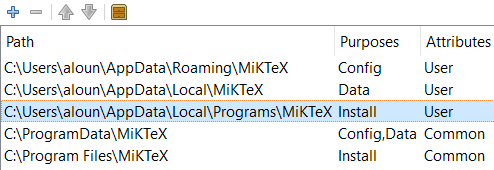
\includegraphics[width=0.7\textwidth]{directories}
\end{center}
On macOS, this directory will be 
\begin{verbatim}
	/Users/<user_name>/Library/Application Support/MiKTeX/texmfs/install
\end{verbatim}
Then, place the \opt{package-name} folder under \texttt{tex -> latex}, and under \texttt{Tasks} on the menubar, select \textbf{Refresh file name database}. You should now be able to use commands from \opt{package-name} in any \texttt{tex} file without having to put the \texttt{sty} file in the same location. \p
It would be wise to pin the file or folder containing your commands to VS Code's icon and the File Explorer icon on your taskbar for easy access. 

\subsection{Images: \texttt{graphicx}} \label{subsec:images}
A picture of black writing on a whiteboard with the \textbf{shadows}, \textbf{contrast}, and \textbf{brightness} maximized, the \textbf{saturation} minimized, and possibly some other settings adjusted as needed---such as increasing the \textbf{brilliance} or slightly increasing the \textbf{exposure}---often gives an image whose white background nearly matches the white page and whose black writing nearly matches the black print. 
\begin{center}
	
\includegraphics[scale=0.1]{whiteboard}
\end{center}
Use the \texttt{center} environment or \verb$\centering$ if it's in a \texttt{figure} environment.\footnote{
	For subfigures, consider using the \texttt{subfigure} environment from the \texttt{subcaption} package. 
}\textsuperscript{,}\footnote{
	The option \texttt{[h]} stands for ``here'' and indicates that we want the figure to be placed exactly where it is in the code. Sometimes this is not enough, and stronger options are required. Ordered by strength, these are \texttt{[h] $<$ [!h] $<$ [H]}, where \texttt{H} comes from the \texttt{float} package.
}
\begin{figure}[H]
	\centering
	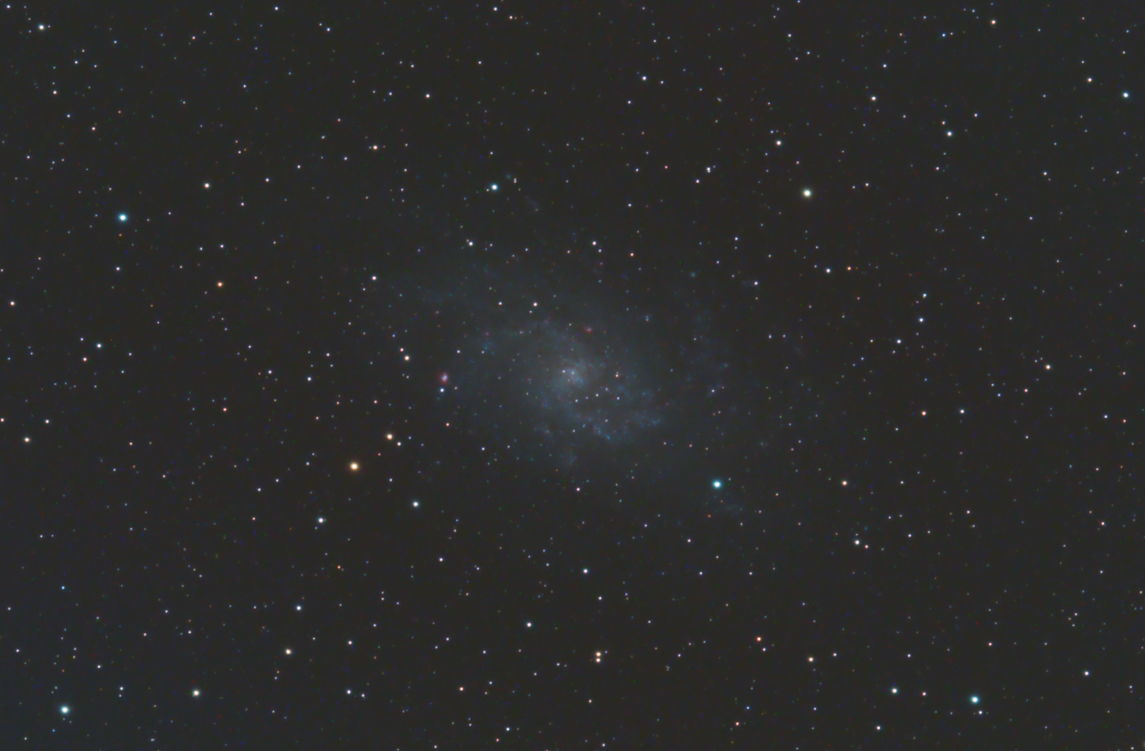
\includegraphics[width=0.75\textwidth]{M33_figure}
	\caption{M33}
\end{figure}
\noindent
Set the path to the folder with your images with \verb$\graphicspath{{$\opt{path}\verb$}}$. \\
The file extensions of the images aren't required. \\
The \texttt{graphicx} package allows us to easily size images with \texttt{scale}, \texttt{width}, or \texttt{height}. Compare the options of the two images above. 

\subsection{Diagrams: PGF/Ti\textit{k}Z} \label{subsec:graphics}
The \texttt{pgf} and \texttt{tikz} packages provide a very complex set of commands to draw shapes, graphs, and intricate diagrams straight into the document. 
You will probably never need to use them, but as before, your best resource for learning PGF/Ti\textit{k}Z is the internet, so look for a some tutorials that might be helpful such as \href{https://www.overleaf.com/learn/latex/LaTeX_Graphics_using_TikZ:_A_Tutorial_for_Beginners_(Part_1)%E2%80%94Basic_Drawing}{this}. \par
Many packages and Ti\textit{k}Z libraries build off of Ti\textit{k}Z so that we can use it for specific tasks without doing all the work. For examples, there are the \href{https://ctan.org/pkg/forest}{\texttt{forest}}, \href{https://ctan.org/pkg/chessboard?lang=en}{\texttt{chessboard}}, and \href{https://ctan.org/pkg/tikzducks}{\texttt{tikzducks}} packages. \par
Note that in the \LaTeX\ menu on the left sidebar in VS Code, under the same Snippet panels mentioned in \S\ref{subsec:formatting-math}, there are Ti\textit{k}Z panels that offer the opportunity to play around with various features from PGF/Ti\textit{k}Z. 

\subsubsection{Chemistry and Physics in \LaTeX} \label{subsubsec:chemistry}
It may perhaps be worth mentioning that there are ways of typesetting other diagrams from the natural sciences in \LaTeX. \\
Click \href{https://en.wikibooks.org/wiki/LaTeX/Chemical_Graphics}{here} for \textbf{general info} on chemical graphics. \\
Click \href{https://tex.stackexchange.com/questions/145838/typesetting-chemical-formulas}{here} for more info on typesetting \textbf{chemical formulas}. \\
Click \href{https://www.overleaf.com/learn/latex/chemistry_formulae}{here} for more info on typesetting \textbf{structural formulas}. \\
Click \href{https://www.overleaf.com/learn/latex/Molecular%20orbital%20diagrams}{here} for info on typesetting \textbf{molecular orbital diagrams}. \\
Click \href{https://www.overleaf.com/learn/latex/Feynman_diagrams}{here} for info on typesetting \textbf{Feynman diagrams}. 

\subsection{Algorithms and Code in \LaTeX} \label{subsec:algorithms}
The \texttt{verbatim} environment prints your code onto the document exactly how it appears in the editor, but it doesn't include tabs. To remedy this, use either the \texttt{Verbatim} environment in the \href{https://ctan.org/pkg/fancyvrb}{\texttt{fancyvrb}} package or the \texttt{verbatimtab} environment in the \href{https://ctan.org/pkg/moreverb}{\texttt{moreverb}} package. Both produce the same result: 
\begin{Verbatim}
SumArrayElements(A[1..n])
num <- 0
FOR i <- 1 to n DO
	num <- num + A[i]
end FOR
RETURN num 
\end{Verbatim}
However, there are better options from other packages shown \href{https://en.wikibooks.org/wiki/LaTeX/Algorithms}{here} and \href{https://en.wikibooks.org/wiki/LaTeX/Source_Code_Listings}{here}. 
\end{document}